\documentclass[../problems.tex]{subfiles}

\graphicspath{{../images/}}

\begin{document}

\section{Projectiles and Charged Particles}
\barh

\paragraph{2.1}
The ratio of the quadratic and linear terms of drag is
\begin{equation*} \tag{2.7}
    \frac{f_q}{f_l} = \frac{cv^2}{bv} = \frac{\gamma D}{\beta} v = [ \qty{1.6e3}{\s  \per \m^2}] Dv
\end{equation*}
where $\beta = \qty{1.6e-4}{\N.\s\per\m^2}$ and $\gamma = \qty{0.25}{\N.\s^2\per\m^4}$ for spherical
projectiles at STP. When $f_q/f_l = 1$ both drag forces are equally important.
\barh
For the baseball $D = 7 \si{cm}$ 
\begin{align*}
    1 &= \qty{1.6e3}{\s  \per \m^2} Dv \\
    v &= \frac{1}{\qty{1.6e3}{\s  \per \m^2} D} \\
    v &= \frac{1}{\qty{1.6e3}{\s  \per \m^2} (\qty{0.07}{\m})} \\
    v &= \qty{0.9}{\frac{\cm}{\s}}
\end{align*}

For the beach ball $D = 70 \si{cm}$
\begin{align*}
    v &= \frac{1}{\qty{1.6e3}{\s  \per \m^2} \qty{0.7}{\m}} \\
    &= \qty{0.9}{\frac{\mm}{\s}}
\end{align*}

The linear term is negligible when $f_q/f_l \gg 1$.

\paragraph{2.2}
From Stokes's law, the viscous drag on a sphere is
\begin{equation*} \tag{2.82}
    f_{lin} = 3\pi \eta D v
\end{equation*}
At STP $\eta = \qty{1.7e-5}{\N.\s\per\m^2}$
\barh
From (2.3) and (2.4)
\begin{align*}
    f_{lin} &= 3\pi \eta D v \\
    bv &= 3\pi \eta D v \\
    \beta D v &= 3\pi \eta D v \\
    \beta &= 3\pi \eta \\
    \beta &= \qty{1.6e-4}{\N.\s\per\m^2}
\end{align*}

\paragraph{2.3}
(a) Show ratio of drag can be written as $f_q/f_l = R/48$ for a sphere of radius $R$ is Reynolds'
number
\begin{equation*}
    \tag{2.83}
    R = \frac{DvQ}{\eta}
\end{equation*}

(b) Find $R$ for a steel ball bearing $D = 2 \si{\mm}$, $ v = 5 \si{\cm\per\s}$, 
$Q = 1.3 \si{\g\per\cm^3}$, and $\eta = \qty{12}{\N.\s\per\m^2}$
\barh
(a) For a sphere $K = 1/4$ and the surface of the swept cross section of a sphere $A = \pi D^2/4$.
Substituting (2.84) and (2.82)
\begin{align*}
    \frac{f_q}{f_l} = \frac{K Q A v^2}{3\pi \eta D v} = \frac{1/4 Q \frac{\pi D^2}{4}v}{3\pi\eta D}
    = \frac{1}{48}\frac{DvQ}{\eta} = \frac{R}{48}
\end{align*}

(b) From (2.83)
\begin{equation*}
    R = \frac{0.002(0.05)(1300)}{12} = 0.011
\end{equation*}

\paragraph{2.4}
(a) Show that the rate (mass/time) is $QAv$ for quadratic drag (b) Show the net force of drag is
$F_d = QAv^2$ (c) Given
\begin{equation*}
    \tag{2.84} \label{eq2.84}
    f_q = KQAv^2 
\end{equation*}
Show (2.84) $\rightarrow$ (2.3) and verify $\gamma$ from (2.4) given the density of air at STP is
 $Q = 1.29 \si{\kg\per\m^3}$ and $K = 1/4$ for a sphere.
\barh

(a) The volume of the fluid swept by the projectile is $v_{swept} = Avt$ where $A$ is the cross
sectional area of the projectile. The mass of the fluid swept is $m_f = Qv_{swept} = QAvt$. The rate
at which the projectile encounters the fluid is the time derivative $\dv{m_f}{t} = QAv$.

(b) The net force of drag is equivalent to the time derivative of momentum of the fluid swept by the
projectile. As the fluid is accelerated from rest to velocity $v$ the change in momentum is
\begin{equation*}
    \dv{p}{t} = \dv{m_f}{t} v + m_f \dv{v}{t} = QAv^2
\end{equation*}

(c) \eqref{eq2.84} in the form of (2.3) is shown as
\begin{equation*}
    f_q = KQAv^2 = cv^2
\end{equation*}
Where the constant $c = KQA$. Substituting $c$ into (2.4)
\begin{align*}
    \gamma D^2 &= KQA
\end{align*}
The cross sectional area of a sphere is $A = \pi D^2/4$ so
\begin{align*}
    \gamma D^2 &= KQ\frac{\pi D^2}{4} \\
    \gamma &= \frac{KQ\pi}{4} \\
    \gamma &= \frac{\qty{1.29}{\kg \per \m^3} \pi}{16} \\
    \gamma &= \qty{0.253}{\N.\s^2\per\m^4}
\end{align*}

\paragraph{2.5} Describe a projectile subject to linear drag is thrown vertically down where
$v_{yo} > v_t$.
Plot $v_y$ vs $t$ for $v_{yo} = 2 v_t$ 
\barh
While $v_y > v_t$ the drag force is larger than the magnitude of weight and the projectile slows
down at an exponential rate until it reaches terminal velocity.
For when $v_{yo} = 2 v_t$, using (2.30) the equation of motion is
\begin{equation*}
    v_y = v_t + (2v_t - v_t)e^{t/\tau} = v_t(1 + e^{-t/\tau})
\end{equation*}

\begin{figure}[h]
    \centering
    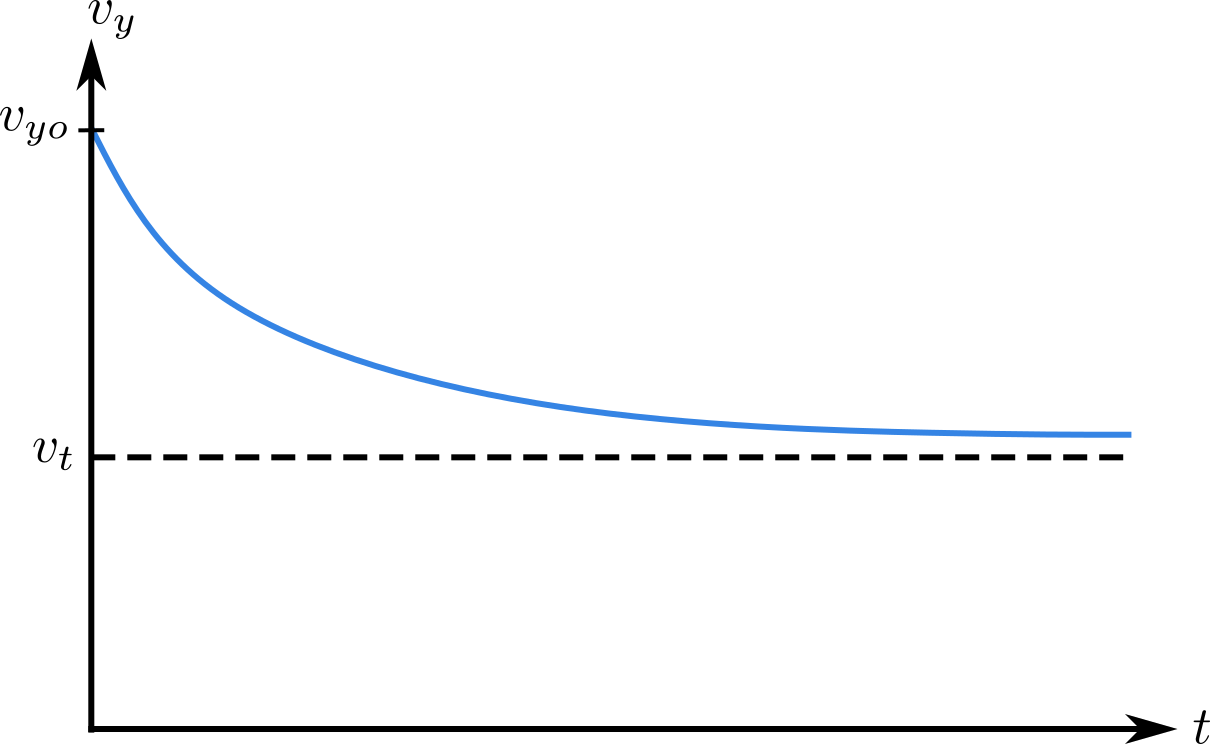
\includegraphics[width=0.5\linewidth]{fig2_5.png}
    \caption{Plot of $v_y$ vs $t$ for $v_{yo} = 2 v_t$}
    \label{fig:2_5}
\end{figure}

\paragraph{2.7} For the motion of a one-dimensional particle subject to a force that depends only on
velocity, $F = F(v)$. Newton's second law $F = m \dv{v}{t}$ is rewritten as $m\:\dd v/F(v) = \dd t$.
Integrating both sides gives
\begin{equation*}
    t = m \int_{v_0}^v \frac{dv'}{F(v')}
\end{equation*}
\barh
For the special case of a constant $F(v) = F_o$
\begin{align*}
    t &= m \int_{v_0}^v \frac{dv'}{F_o} \\
    t &= \frac{m}{F_o} \int_{v_0}^v dv' \\
    t &= \frac{m}{F_o} (v-v_o) \\
    v &= v_o + \frac{F_o}{m} t
\end{align*}

This is the first of the SUVAT equations where $a = F_o/m$.

\paragraph{2.9} Using seperation of variables (2.29) is rewritten as
\begin{equation*}
    \frac{m \: dv_y}{v_y - v_t} = -b dt
\end{equation*}
\barh 
Integrating both sides from time 0 to $t$
\begin{align*}
    \int_0^t \frac{m \: dv_y}{v_y - v_t} &= -b \int_0^t dt \\
    m \int_{v_{yo}}^{v_y} \frac{dv_y'}{v_y' - v_t} &= -bt \\
    m \ln \abs{\frac{v_y - v_t}{v_{yo} - v_t}} &= -bt \\
    \ln \abs{\frac{v_y - v_t}{v_{yo} - v_t}} &= -\frac{bt}{m} \\
    \abs{\frac{v_y - v_t}{v_{yo} - v_t}} &= e^{-t/\tau} \\
    v_y &= v_t + (v_{yo} - v_t)e^{-t/\tau}
\end{align*}
where $\tau = m/b$ and $v_y = v_{yo}$ when $t = 0$. This is the same as (2.30). 

\paragraph{2.11} An object is thrown vertically upward with initial velocity $v_{o}$ in a linear
medium. (a) Measuring \textit{y upward}, write $v_y(t)$ and $y(t)$. (b) Find the time at $y_{max}$.
(c) Show $y_{max} = v_{o}^2/2g$ as the drag coefficient approaches zero. [\textit{Hint:} Use the
Taylor series approximation $\ln (1 + \delta) \approx \delta - \frac{1}{2}\delta^2$ for large $v_t$]
\barh 
% figure for 2_11
\begin{figure}[ht]
    \centering
    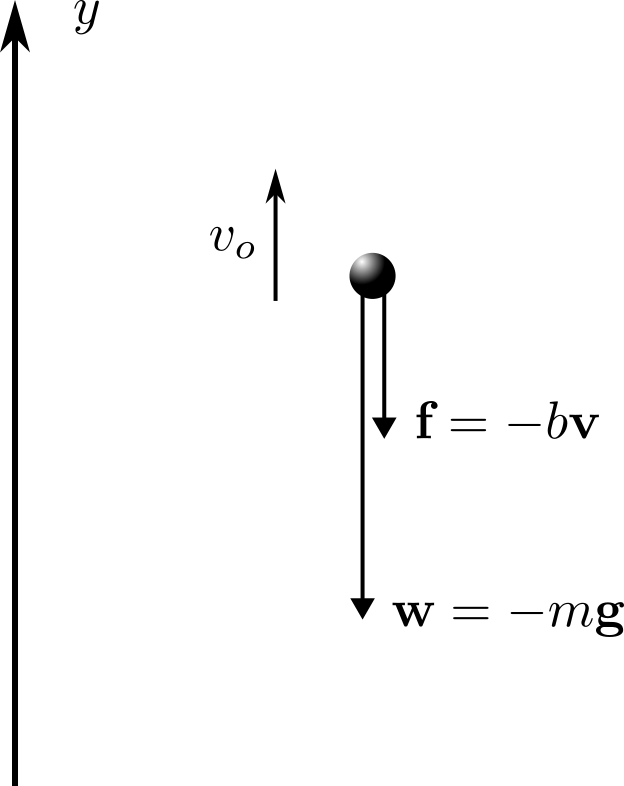
\includegraphics[scale=1]{fig2_11.png}
    \caption{Free body diagram of an object thrown vertically upward with initial velocity $v_o$.}
    \label{fig:2_11}
\end{figure}
(a) The equation of motion is
\begin{align*}
    m \dot{v}_y &= -mg - b v_y \\
    m \dot{v}_y &= -b(v_y + v_t)\\
    m \frac{\dd{v_y}}{v_y + v_t} &= -b \dd{t} \\
    m \int_{v_{o}}^{v_y} \frac{\dd{v_y'}}{v_y' + v_t} &= -b \int_0^t \dd{t'} \\
    m \ln \abs{\frac{v_y + v_t}{v_{o} + v_t}} &= -bt \\
    \frac{v_y + v_t}{v_{o} + v_t} &= e^{-t/\tau} \\
    v_y &= -v_t + (v_{o} + v_t)e^{-t/\tau}
\end{align*}
This is the same as (2.30) but $v_t$ has a reversed sign. The position is (2.35) with $v_t$
replaced by $-v_t$
\begin{equation*}
    y(t) = -v_t t + (v_{o} + v_t) \tau (1 - e^{-t/\tau})
\end{equation*}
(b) The time at $y_{max}$ is found by setting $v_y = 0$ and solving for $t$
\begin{align*}
    0 &= -v_t + (v_{o} + v_t)e^{-t/\tau} \\
    \frac{v_t}{v_{o} + v_t} &= e^{-t/\tau} \\
    \ln (\frac{v_t}{v_{o} + v_t}) &= -\frac{t}{\tau} \\
    t &= -\tau \ln (\frac{v_t}{v_{o} + v_t}) \\
    t_{max} &= \tau \ln (1 + \frac{v_{o}}{v_t})
\end{align*}
Substituting the time at the highest point into $y(t)$ gives the maximum height
\begin{align*}
    y(t_{max}) &= -v_t t_{max} + (v_{o} + v_t) \tau (1 - e^{-t_{max}/\tau}) \\
    y_{max} &= -v_t \tau \ln (1 + \frac{v_{o}}{v_t}) + (v_{o} + v_t) \tau 
        \quantity[1 - e^{-\ln (1 + \frac{v_{o}}{v_t})}] \\
    &= -v_t \tau \ln (1 + \frac{v_{o}}{v_t}) + (v_{o} + v_t) \tau 
        \quantity[1 - \frac{v_t}{v_{o} + v_t}] \\
    y_{max} &= \tau \quantity[-v_t \ln (1 + \frac{v_{o}}{v_t}) + v_{o}] 
\end{align*}
(c) When the drag force is small $v_o/v_t$ is very small, so using the Taylor series approximation
\begin{align*}
    y_{max} &= \tau\quantity[-v_t \quantity[\frac{v_o}{v_t} 
        - \frac{1}{2}\quantity(\frac{v_o}{v_t})^2] + v_{o}] \\
    &= \tau\quantity[\frac{v_o^2}{2v_t}] \qgiven{v_t = g\tau} \\ 
    y_{max} &= \frac{v_o^2}{2g}
\end{align*}

\paragraph{2.13} A mass $m$ is constained to move on the $x$ axis and subject to a net force
$F(x) = -kx$ where $k$ is a positive constant. The mass is released from rest at $x = x_o$ and
$t = 0$. Find the mass's speed as a function of $x$ given
\begin{equation*}
    \tag{2.85} \label{eq2.85}
    v^2 = v_o^2 + \frac{2}{m} \int_{x_o}^x F(x') \dd{x'}
\end{equation*}
Find $x$ as a function of $t$ through seperation of variables, integrating from time 0 to $t$.
\barh
With initial velocity $v_o = 0$ (2.85) is rewritten as
\begin{equation*}
    v^2 = -\frac{2k}{m} \int_{x_o}^x x'\dd{x'} = \frac{k}{m}(x_o^2 - x^2) 
    \qor v = -\omega \sqrt{x_o^2 - x^2}
\end{equation*}
where $\omega^2 = k/m$, the angular frequency. The sign is negative because the mass is moving in
the negative $x$ direction first due to the force $F(x) = -kx$. Separating variables to find $x(t)$
\begin{align*}
    \frac{-\dd{x}}{\sqrt{x_o^2 - x^2}} &= \omega dt \\
    \int_{x_o}^x \frac{-\dd{x'}}{\sqrt{x_o^2 - x'^2}} &= \omega \int_0^t dt' \\
    \arccos(\frac{x}{x_o}) &= \omega t \\
    x(t) &= x_o \cos(\omega t)
\end{align*}
where the integral comes from the identity ${\dv{u}\arccos(u/a) = \frac{-1}{\sqrt{a^2-u^2}}}$

\paragraph{2.15} A projectile launched with velocity $(v_{xo}, v_{yo})$ with no air resistance.
Show the horizontal range is $2v_{xo}v_{yo}/g$.
\barh 
The equation of motion for the projectile with no drag is $\vb{\ddot r} = \vb g$. Integrating the 
components
\begin{align*}
    \ddot{x} &= 0       & \ddot y &= -g\\ 
    \dot{x} &= v_{xo}   & \dot y &= -gt\\
    x &= v_{xo} t + x_o & y &= -\frac{1}{2}gt^2 + v_{yo}t + y_o \\
    x &= v_{xo} t       & y &= -\frac{1}{2}gt^2 + v_{yo}t
\end{align*}
where we set $x_o = y_o = 0$. The projectile hits the ground at $y = 0$ and solving for $t$
\begin{align*}
    0 &= -\frac{1}{2}gt^2 + v_{yo}t \\
    t_{range} &= \frac{2v_{yo}}{g}
\end{align*}
Substituting $t_{range}$ into $x$
\begin{align*}
    x &= \frac{2v_{xo}v_{yo}}{g}
\end{align*}
which is the horizontal range of the projectile in a vacuum.

\paragraph{2.17} Eliminate $t$ from (2.36) to give $y$ as a function of $x$ verifying (2.37)
\barh 
Solving the first equation of (2.36) for $t$ 
\begin{align*}
    x = v_{xo} \tau \quantity(1 - e ^{-t/\tau}) \\
    e^{-t/\tau} = 1 - \frac{x}{v_{xo} \tau} \\
    -\frac{t}{\tau} = \ln(1 - \frac{x}{v_{xo} \tau}) \\
    t = -\tau \ln (1 - \frac{x}{v_{xo} \tau})
\end{align*}
and substituting into the second equation
\begin{align*}
    y &= (v_{yo} + v_t) \tau \quantity(1 - e ^{-t/\tau}) - v_t t \\
    &= (v_{yo} + v_t)\tau\quantity(1 - 1+\frac{x}{v_{xo}\tau})+v_t\tau\ln(1-\frac{x}{v_{xo}\tau}) \\
    y &= \frac{v_{yo} + v_t}{v_{xo}} x + v_t \tau \ln (1 - \frac{x}{v_{xo} \tau})
\end{align*}
which is the same as (2.37).

\paragraph{2.19} (a) Find $y$ as a function of $x$ for a projectile with no air resistance. (b) Show
that (2.37) reduces to part (a) when air resistance is switched off($\tau$ and $v_t$ approach
infinity). [\textit{Hint:} Use the Taylor series approximation for $\ln(1 - \epsilon)$]
\barh
(a) A projectile with no air resistance has position $\vb r = (x, y) = (v_{xo}t, v_{yo}
t - \frac{1}{2}gt^2)$. To find $y$ as a function of $x$, subsitute $t = x/v_{xo}$ into $y$
\begin{align*}
    y &= v_{yo} \frac{x}{v_{xo}} - \frac{1}{2}g \frac{x^2}{v_{xo}^2} \\
    y &= \frac{v_{yo}}{v_{xo}} x - \frac{1}{2}g \frac{x^2}{v_{xo}^2}
\end{align*}
(b) Using the Taylor series approximation for $\ln(1 - \epsilon)$
\begin{align*}
    \ln(1- \frac{x}{v_{xo} \tau}) &= -\frac{x}{v_{xo} \tau} - \frac{1}{2} \frac{x^2}{v_{xo}^2
        \tau^2} \\
\end{align*}
Substituting into (2.37)
\begin{align*}
    y &= \frac{v_{yo} + v_t}{v_{xo}} x + v_t \tau \quantity(-\frac{x}{v_{xo} \tau} - \frac{1}{2}
        \frac{x^2}{v_{xo}^2 \tau^2})  \\
    &= \frac{v_{yo} + v_t}{v_{xo}} x - v_t \frac{x}{v_{xo}} - \frac{1}{2} \frac{v_t}{v_{xo}^2}
        \frac{x^2}{\tau} \\
    &= \frac{v_{yo}}{v_{xo}} x - \frac{1}{2} \frac{v_t}{v_{xo}} \frac{x^2}{\tau} \qusing 
        {v_t = g\tau} \\
    y &= \frac{v_{yo}}{v_{xo}} x - \frac{1}{2} g \frac{x^2}{v_{xo}^2} \\
\end{align*}

\paragraph{2.21} Ignoring air resistance, use cylindrical polar coordinates to show
\begin{equation*}
    z = \frac{v_o^2}{2g} - \frac{g}{2v_o^2} \rho^2
\end{equation*}
\barh
% figure of 2_21a
\begin{figure}[ht]
    \centering
    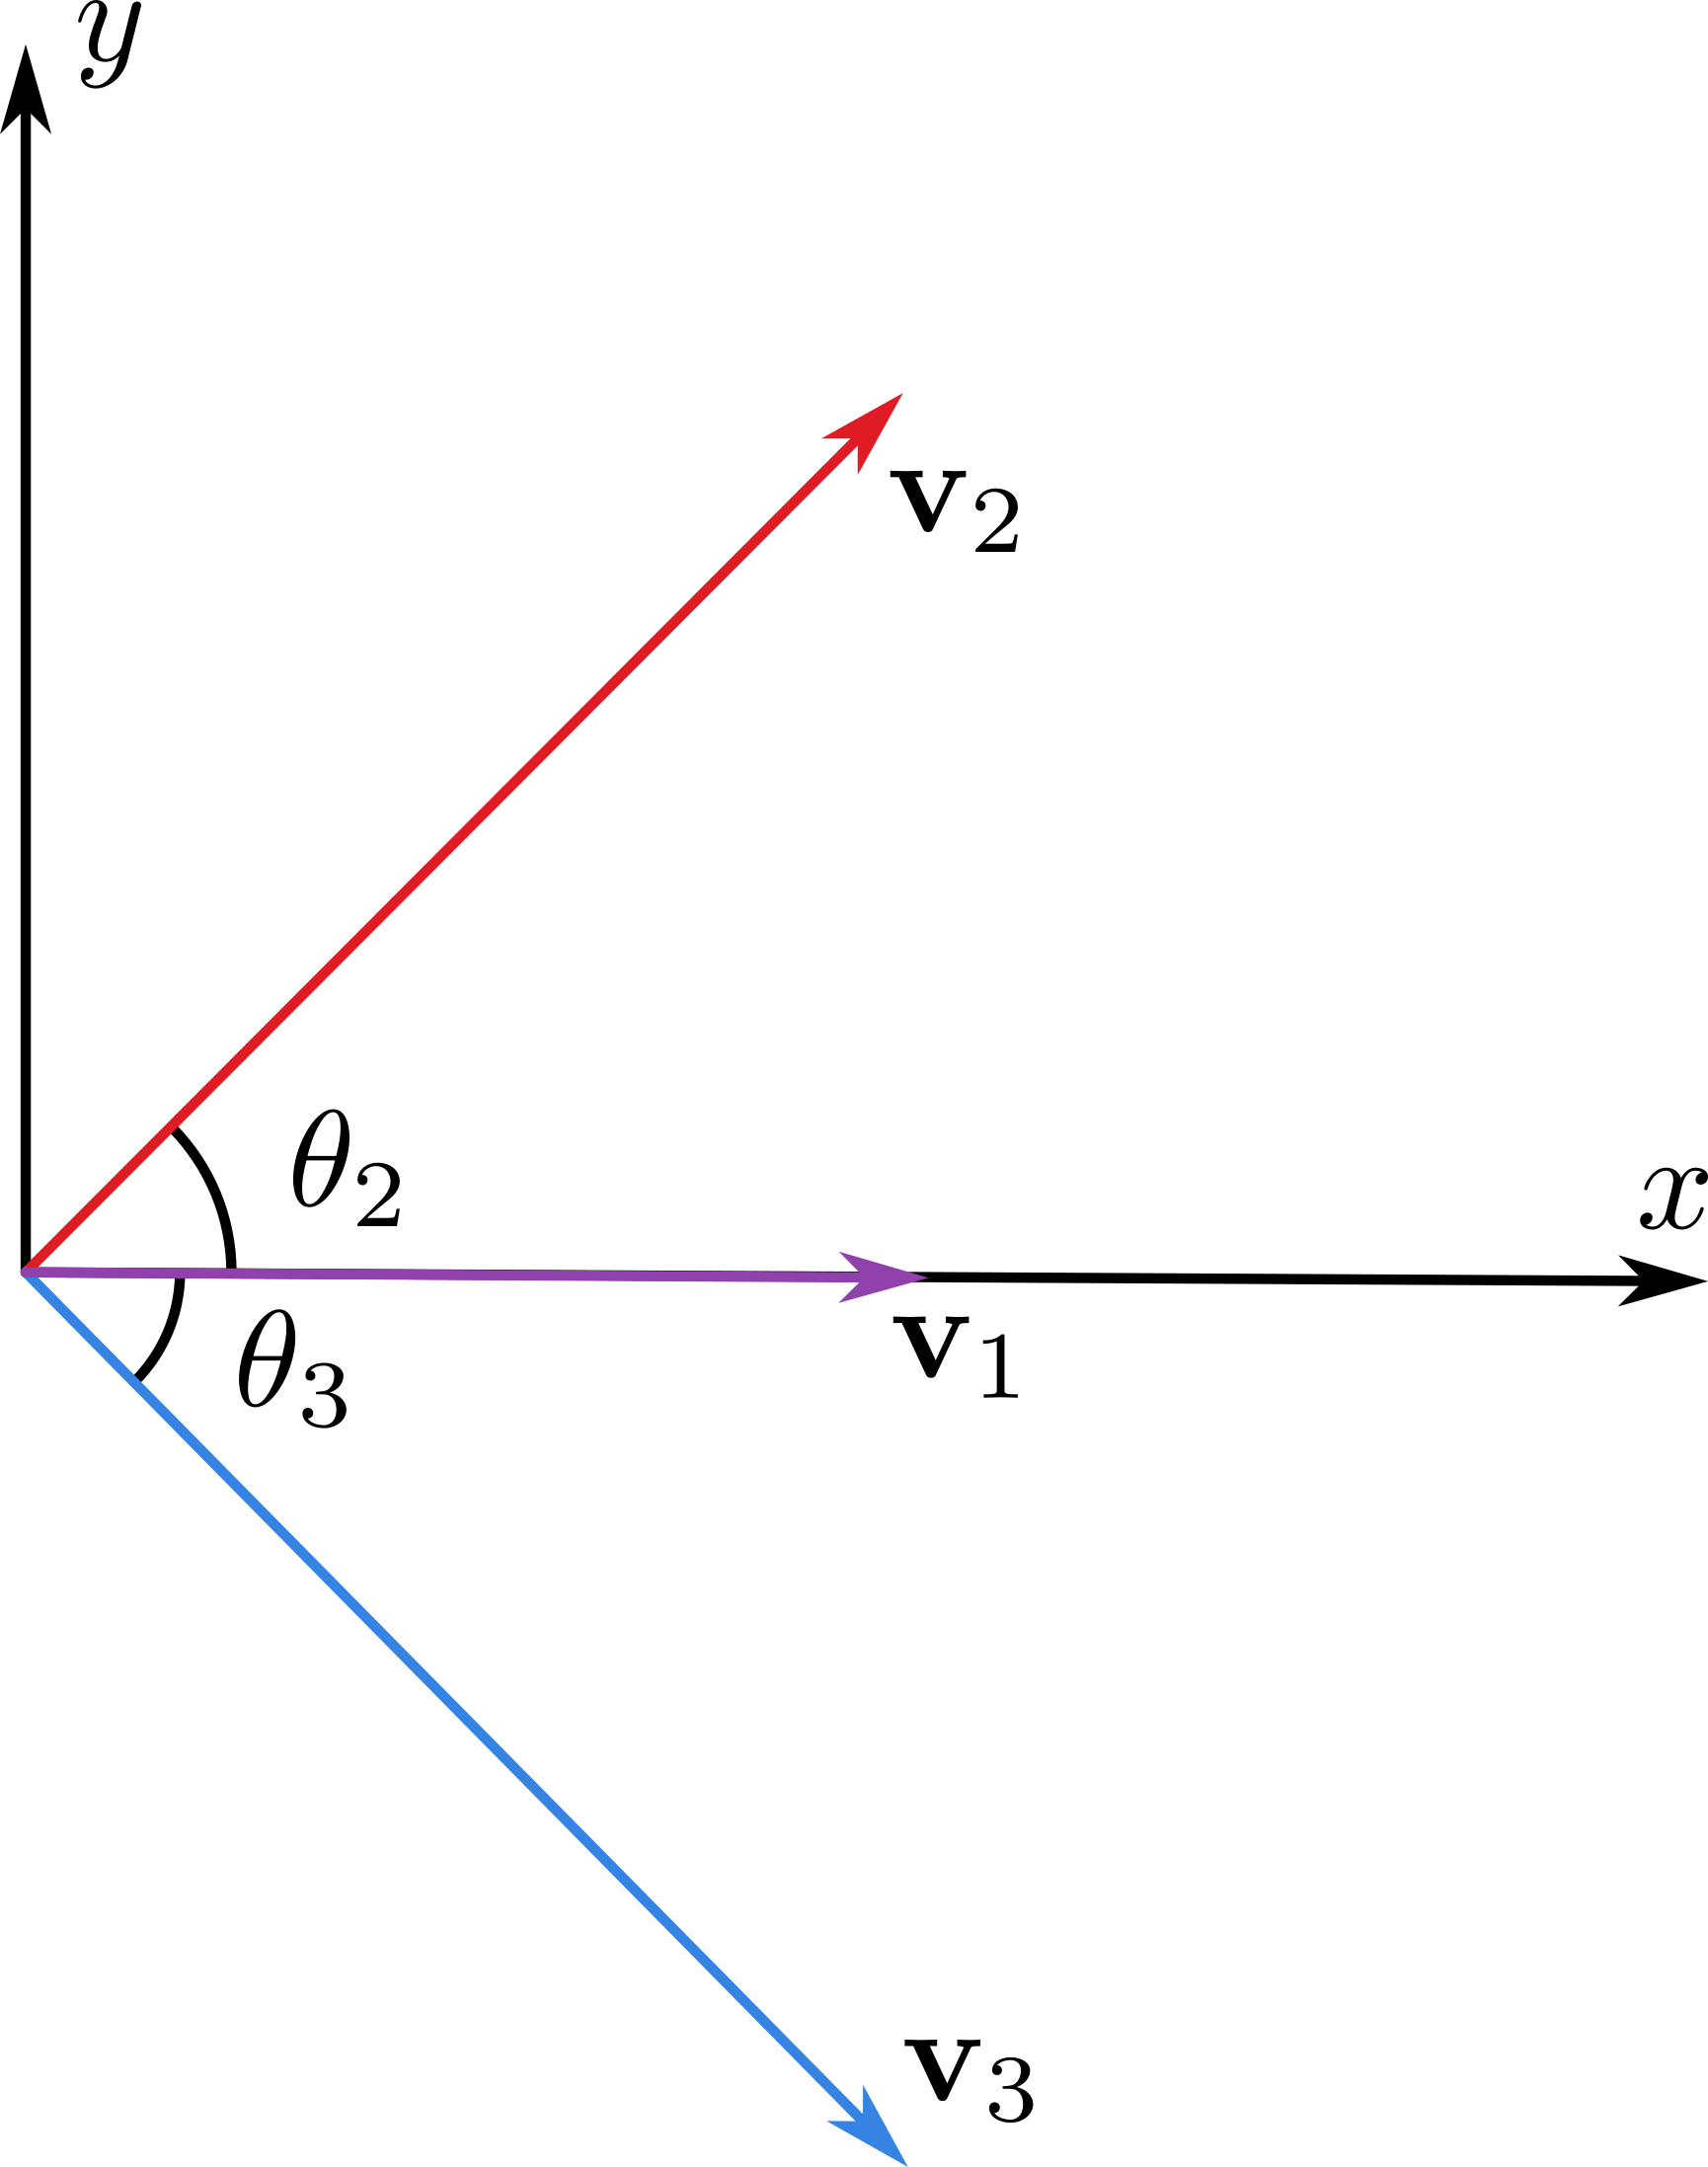
\includegraphics[scale=1]{fig2_21a.png}
    \caption{Projectile from gun at angle $\theta$ above the horizontal.}
    \label{fig:2_21a}
\end{figure}
Setting $\phi = 0$ and $z = 0$ at $t = 0$, the projectile is fired at an angle $\theta$ above the
horizontal. From velocity is $v_{\rho o} = v_o \cos \theta, v_{zo} = v_o \sin \theta$. Solving the
equations of motion
\begin{align*}
    \ddot \rho &= 0             & \ddot z &= -g \\
    \dot{\rho} &= v_{\rho o}    & \dot{z} &= v_{zo} - gt \\
    \rho &= v_o t \cos \theta   & z &= v_o t\sin \theta - \frac{1}{2}gt^2 \\
\end{align*}
Substituting $t = \rho/v_{\rho o}$ into $z$
\begin{align*}
    z &= v_o \frac{\rho}{v_{\rho o}} \sin \theta - \frac{1}{2}g \frac{\rho^2}{v_{\rho o}^2} \\
    z &= \rho \tan \theta - \frac{1}{2}g \frac{\rho^2}{v_o^2} \sec^2 \theta \\
\end{align*}
Taking the derivative of $z$ with respect to $\theta$ and setting it equal to zero to find the maximum
height.
\begin{align*}
    \dv{z}{\theta} &= \rho \sec^2\theta - \frac{1}{2}g\frac{\rho^2}{v_o^2} 2\sec^2\theta\tan\theta\\
    0 &= \rho \sec^2\theta(1 - \frac{g\rho}{v_o^2} \tan\theta) \\
    \tan \theta &= \frac{v_o^2}{g\rho}
\end{align*}
Substituting $\theta$ into $z$
\begin{align*}
    z &= \rho \frac{v_o^2}{g\rho} - \frac{1}{2}g \frac{\rho^2}{v_o^2} (1 + \tan^2\theta) \\
    z &= \frac{v_o^2}{2g} - \frac{g}{2v_o^2} \rho^2
\end{align*}
where the maximum height is $z_{max} = v_o^2/2g$.

\paragraph{2.23} Find the terminal speeds in air of (a) steel ball bearing $D = \qty{3}{\mm}$, (b)
16 pound steel shot, and (c) 200 pound parachutist in free fall in the fetal position. Assume drag
is purely quadratic. Density of steel is $\qty{8}{\g\per\cm^3}$ and the parachutist is a sphere of
density $\qty{1}{\g\per\cm^3}$.
\barh 
The terminal speed is given by
\begin{equation*}
    v_t = \sqrt{\frac{mg}{\gamma D^2}}
\end{equation*}
where mass $m$ is given by the density $m = QV$ and $V = \pi D^3/6$ for a sphere. The new equation
for terminal speed is
\begin{equation*}
    v_t = \sqrt{\frac{QVg}{\gamma D^2}} = \sqrt{\frac{Q\pi D g}{6\gamma}}
\end{equation*}
for an unknown diameter, solve for $D$ from the density $Q = m/V$
\begin{equation*}
    D = \quantity(\frac{\pi Q}{6m})^{1/3}
\end{equation*}
and substitute into the equation for terminal speed
\begin{equation*}
    v_t = \sqrt{\frac{m g}{\gamma}} \quantity(\frac{\pi Q}{6m})^{1/3}
\end{equation*}
(a) Using the diameter $D = \qty{0.003}{\m}$, density of steel $Q = \qty{8}{\g\per\cm^3}$, and
$\gamma = \qty{0.25}{\N.\s^2\per\m^4}$, the terminal speed is
\begin{align*}
    v_t &= \sqrt{\frac{Q\pi D g}{6\gamma}} \\
    &= \sqrt{\frac{\qty{8000}{\kg\per\m^3} \cdot \pi \cdot \qty{0.003}{\m} \cdot 
        \qty{9.8}{\m\per\s^2}}{6\cdot\qty{0.25}{\N.\s^2\per\m^4}}} \\
    &= \qty{22}{\m/\s} 
\end{align*}
(b) For a steel shot $m = \qty{7.26}{\kg}$, $Q = \qty{8000}{\kg\per\m^3}$, the terminal speed is
\begin{equation*}
    v_t = \sqrt{\frac{\qty{7.26}{\kg}\cdot\qty{9.8}{\m/\s^2}}{\qty{0.25}{\N.\s^2\per\m^4}}}
        \quantity(\frac{\pi\qty{8000}{\kg/\m^3}}{6\cdot\qty{7.26}{\kg}})^{1/3} = \qty{140}{\m/\s}
\end{equation*}
(c) For a parachutist $m = \qty{91}{\kg}$, $Q = \qty{1000}{\kg\per\m^3}$, the terminal speed is
\begin{equation*}
    v_t = \sqrt{\frac{\qty{91}{\kg}\cdot\qty{9.8}{\m/\s^2}}{\qty{0.25}{\N.\s^2\per\m^4}}}
        \quantity(\frac{\pi\qty{1000}{\kg/\m^3}}{6\cdot\qty{91}{\kg}})^{1/3} = \qty{107}{\m/\s}
\end{equation*}

\paragraph{2.25} For horizontal motion under quadratic drag, derive the results of (2.49) and (2.51)
and verify the constant $\tau=m/cv_o$ is time.
\barh 
The equation of motion for horizontal motion under quadratic drag is
\begin{equation*}
    m \dv{v}{t} = -c v^2
\end{equation*}
Separating variables and integrating
\begin{align*}
    \int_{v_o}^v \frac{m \dd{v'}}{v'^2} &= -c \int_0^t \dd{t'} \\
    \frac{m}{v_o} - \frac{m}{v} &= -ct \\
    \frac{1}{v} &= \frac{1}{v_o} + \frac{ct}{m} \\
    v &= \frac{v_o}{1 + \frac{cv_ot}{m}} = \frac{v_o}{1 + t/\tau}
\end{align*}
Integrating again to find $x$ from time 0 to $t$
\begin{align*}
    \int_0^x \dd{x'} &= \int_0^t \frac{v_o}{1 + t'/\tau} \dd{t'} \\
    x &= v_o \tau \ln (1 + \frac{t}{\tau}) 
\end{align*}
Verifying the constant $\tau = m/cv_o$ using dimensional analysis: The unit of coefficient $c$
is
\begin{equation*}
    [c] = \quantity[\frac{F}{v^2}] = \frac{\si{M.L\per T^2}}{\si{L^2/T^2}} = \si{M.L^{-1}}  
\end{equation*}
and with $[m] = \si{M}$ and $[v_o] = \si{L/T}$, the unit of $\tau$ is
\begin{equation*}
    [\tau] = \frac{\si{M}}{\si{M.L^{-1}} \cdot \si{L/T}} = \si{T}
\end{equation*}

\paragraph{2.27} Write Newton's second law for a particle of mass $m$ sliding up a frictionless
incline of angle $\theta$ with the horizontal and subject to quadratic drag and solve for $v$ as a
function of $t$. How long does the upward journey last?
\barh
The equation of motion is
\begin{equation*}
    m \dot{v} = -mg \sin \theta - c v^2 = -c (v_t^2 + v^2)
\end{equation*}
where $v_t^2 = mg\sin\theta/c$. Separating variables and integrating
\begin{align*}
    \int_{v_o}^v \frac{m \dd{v'}}{v_t^2 + v'^2} &= -c \int_0^t \dd{t'} \\
    \frac{m}{v_t} [\arctan(v/v_t) - \arctan(v_o/v_t)]&= -ct \\
    \arctan(v/v_t) - \arctan(v_o/v_t) &= -\frac{cv_ot}{m} \\
    v &= v_t \tan(\arctan(v_o/v_t) - \frac{cv_ot}{m})
\end{align*}
The time it takes to reach the top of the incline is when $v = 0$ and solving for $t$
\begin{align*}
    0 &= \arctan(v_o/v_t) - \frac{cv_ot}{m} \\
    t &= \frac{m}{cv_o} \arctan(v_o/v_t)
\end{align*}

\paragraph{2.29} Compare the speeds of a skydiver subject to quadratic drag who has a terminal speed
of $\qty{50}{\m/\s}$ for times $t = \numlist{1;5;10;20;30}$ seconds.
\barh 
The equation of motion for a skydiver subject to quadratic drag is
\begin{equation*}
    m \dot{v} = -mg - cv^2
\end{equation*}
where $v_t^2 = mg/c$. Separating variables and integrating gives 
\begin{equation*} \tag{2.57}
    v(t) = v_t \tanh(gt/v_t)
\end{equation*}
In a vacuum the equation for velocity is $v_c(t) = gt$.
% table of values

\begin{center}
    \begin{tabular}{c c c}
        $t$ & $v(t)$ & $v_c(t)$ \\
        \hline
        1 & 9.7 & 9.8 \\
        5 & 38 & 49 \\
        10 & 48 & 98 \\
        20 & 49.96 & 196 \\
        30 & 49.999 & 294
    \end{tabular}
\end{center}

\paragraph{2.31} (a) Find the terminal speed of a basketball of diameter $D=\qty{0.24}{\m}$ and mass
$m=\qty{0.6}{\kg}$. \newline (b) How long does it take to hit the ground from a height of
$h=\qty{30}{\m}$ and what is its speed at impact?
\barh 
(a) Assuming quadratic drag, the terminal speed is
\begin{align*}
    v_t &= \sqrt{\frac{mg}{\gamma D^2}} \\
    &= \sqrt{\frac{\qty{0.6}{\kg} \cdot \qty{9.8}{\m/\s^2}}{\qty{0.25}{\N.\s^2\per\m^4} \cdot 
        0.24^2\si{\m}^2}} \\
    &= \qty{20.2}{\m/\s}
\end{align*}
(b) Solving (2.58) for $t$ when $y = \qty{30}{\m}$ and $v_t = \qty{20.2}{\m/\s}$
\begin{equation*}
    t = \frac{v_t}{g} \arccosh\quantity(e^{gy/v_t^2}) 
        = \frac{\qty{20.2}{\m/\s}}{\qty{9.8}{\m/\s^2}} \arccosh\quantity(e^{\qty{9.8}{\m/\s^2} 
        \cdot \qty{30}{\m} / 20.2^2\si{\m/\s}^2})  = \qty{2.78}{\s}
\end{equation*}
The speed at impact is given by (2.57)
\begin{equation*}
    v(t) = v_t \tanh(gt/v_t) = \qty{20.2}{\m/\s} \tanh(\qty{9.8}{\m/\s^2} \cdot \qty{2.8}{\s} 
        / \qty{20.2}{\m/\s}) = \qty{17.6}{\m/\s}
\end{equation*}
In a vacuum the time to hit the ground is $t = \sqrt{2y/g} = \qty{2.47}{\s}$ and the speed is
$v = \sqrt{2gy} = \qty{25.3}{\m/\s}$.

\paragraph{2.33} (a) Sketch the hyperbolic functions
\begin{equation*}
    \cosh z = \frac{e^z + e^{-z}}{2} \qand \sinh z = \frac{e^z - e^{-z}}{2}
\end{equation*}
for any z, real or complex. (b) Show $\cosh z = \cos(iz)$ and the same relation for $\sinh z$. (c)
Find the derivative and integral of $\cosh z$ and $\sinh z$? (d) Show $\cosh^2 z - \sinh^2 z = 1$.
(e) Show that 
\begin{equation*}
 \int{dx/\sqrt{1+x^2}} = \arcsinh x 
\end{equation*}
[\textit{Hint:} Use the substitution $x = \sinh u$ and the identity from (d)]
\barh
% figure of two plots 2_33a and 2_33b
(a) The hyperbolic functions are plotted in Figure \ref{fig:2_33}.
\begin{figure}[ht]
    \begin{subfigure}{0.49\textwidth}
        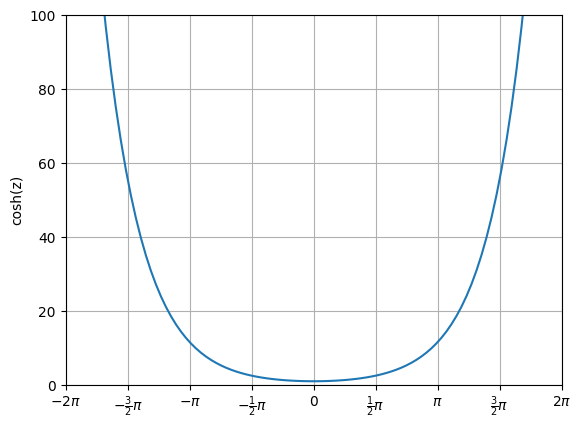
\includegraphics[width=\textwidth]{fig2_33a.png}
        \caption{$y = \cosh z$}
        \label{fig:2_33a}
    \end{subfigure}
    \begin{subfigure}{0.49\textwidth}
        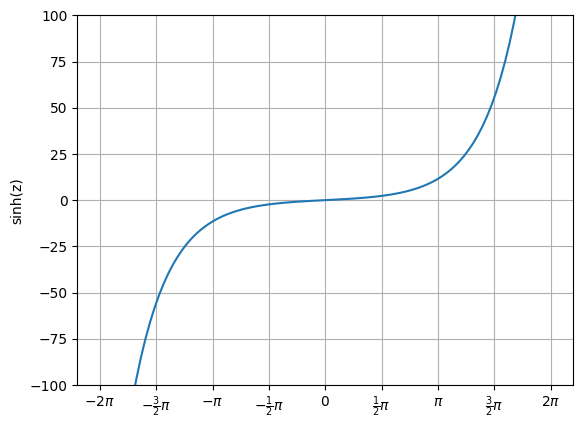
\includegraphics[width=\textwidth]{fig2_33b.png}
        \caption{$y = \sinh z$}
        \label{fig:2_33b}
    \end{subfigure}
    \caption{Graph of hyberbolic functions}
    \label{fig:2_33}
\end{figure}

(b) Using Euler's formula $e^{iz} = \cos z + i \sin z$ the exponents are rewritten as
\begin{equation*}
    e^{i(iz)} = \cos(iz) + i \sin(iz) = e^{-z} \qand e^{-i(iz)} = \cos(iz) - i \sin(iz) = e^z
\end{equation*}
and substituting into the hyperbolic function
\begin{align*}
    \cosh z &= \frac{e^z + e^{-z}}{2} \\
    &= \frac{e^{i(iz)} + e^{-i(iz)}}{2} \\
    &= \cos(iz)
\end{align*}
and the relation for $\sinh z$ is
\begin{align*}
    \sinh z &= \frac{e^z - e^{-z}}{2} \\
    &= \frac{e^{i(iz)} - e^{-i(iz)}}{2} \\
    &= -i \sin(iz)
\end{align*}

(c) The derivative of $\cosh z$ and $\sinh z$ are
\begin{align*}
    \dv{z} \cosh z &= \frac{e^z - e^{-z}}{2} = \sinh z & \dv{z} \sinh z &= \frac{e^z + e^{-z}}{2} 
        = \cosh z
\end{align*}
similarly, the integration gives
\begin{align*}
    \int \cosh z \dd{z} &= \sinh z + C & \int \sinh z \dd{z} &= \cosh z + C
\end{align*}

(d) Using the relation from (b)
\begin{align*}
    \cosh^2 z - \sinh^2 z &= \cos^2(iz) + \sin^2(iz) = 1
\end{align*}

(e) Using the substitution $x = \sinh u$ and the identity from (d)
\begin{align*}
    \int \frac{\dd{x}}{\sqrt{1+x^2}} = \int \frac{\cosh(u)\dd{u}}{\sqrt{1+\sinh^2 u}} 
    = \int \dd{u} = u
    = \arcsinh x  
\end{align*}

\paragraph{2.35} (a) Show the steps from (2.52) to (2.57) and (2.58). (b) Using the parameter
$\tau=v_t/g$, show when $t=\tau$, $v$ is 76\% of the terminal speed. Also show when $t = 2\tau$ and
$3\tau$. (c) Show when $t\gg\tau$, $v\approx v_t t + C$ where $C$ is a constant. (d) Show when $t$
is small, position is $y\approx g t^2/2$.
\barh 
(a) The equation of motion for a particle subject to quadratic drag is
\begin{equation*} \tag{2.52}
    m \dot{v} = mg - cv^2
\end{equation*}
where $v_t^2 = mg/c$. Rewriting (2.52) with the sub $m=v_t^2c/g$
\begin{align*}
    \dot{v} = g - \frac{c}{m} v^2 = g \quantity(1 - \frac{v^2}{v_t^2})
\end{align*}
From seperation of variables and integrating
\begin{align*}
    \frac{1}{1 - v^2/v_t^2}\dd{v} &= g \dd{t} \\
    \int \frac{1}{1 - v'^2/v_t^2}\dd{v'} &= g \int \dd{t'}
\end{align*}
The integral on the left is solved using the u-sub $u = v'/v_t$, $\dd{u} = \dd{v'}/v_t$ and 
$\int 1/(1-u^2) \dd{u}= \arctanh u$
\begin{align*}
    \frac{v_t}{g} \arctanh(v/v_t) &= t
\end{align*}
Solving for $v$ gives
\begin{align*}
    v(t) = v_t \tanh(gt/v_t)
\end{align*}
Integrating again using $\int \tanh u \dd{u} = \ln(\cosh u)$
\begin{align*}
    y(t) = \int v(t) \dd{t} = v_t\int \tanh(gt/v_t) \dd{t} = \frac{v_t^2}{g} \ln(\cosh(gt/v_t))
\end{align*}
(b) Rewriting with the new parameter $\tau$
\begin{align*}
    v(t) = v_t \tanh(t/\tau) \qand y(t) = v_t\tau \ln(\cosh(t/\tau))
\end{align*}
The values of $v(t)$ are
\begin{center}
    \begin{tabular}{c c c}
        $t$ & $v(t)$ & percentage\\
        \hline
        $\tau$ & $\tanh(1)=0.76v_t$ & 76\%\\
        $2\tau$ & $\tanh(2)=0.96v_t$ & 96\%\\
        $3\tau$ & $\tanh(3)=0.995v_t$ & 99.5\%
    \end{tabular}
\end{center}
(c) When $t\gg\tau$, $t/\tau \rightarrow \infty$
\begin{align*}
    v(t) &\approx \lim_{t/\tau \rightarrow \infty}v_t \tanh(t/\tau) = v_t
\end{align*}
and the position is
\begin{align*}
    y(t) \approx \int v(t) \dd{t} = v_t t + C
\end{align*}
(d) When $t$ is small, Using Taylor series approximation for $\ln(1+\delta)\approx\delta$ and 
\begin{align*}
    \cosh x = \frac{e^x + e^{-x}}{2} \approx \frac{1}{2} \quantity(1 + x + x^2/2 + 1 - x + x^2/2)
        = 1 + \frac{x^2}{2} \\ 
\end{align*}
The position is
\begin{align*}
    y(t) &= v_t \tau \ln\quantity[1+\frac{t^2}{2\tau^2}] \\
    &= v_t \tau \quantity[\frac{t^2}{2\tau^2}] \\
    &= \frac{v_t}{2\tau} t^2 \qusing{v_t = g\tau} \\
    y(t) &= \frac{1}{2} gt^2
\end{align*}

\paragraph{2.37} Integrate (2.55) using the partial fraction
\begin{align*}
    \frac{1}{1-u^2} = \frac{1}{2}\quantity[\frac{1}{1+u} + \frac{1}{1-u}]
\end{align*}
\barh 
The integral of the partial fraction is
\begin{align*}
    \int \frac{1}{1-u^2} \dd{u} &= \frac{1}{2} \int \frac{1}{1+u} \dd{u} + \frac{1}{2} \int 
        \frac{1}{1-u} \dd{u} \\
    &= \frac{1}{2} \ln(1+u) - \frac{1}{2} \ln(1-u) + C \\
    &= \frac{1}{2} \ln\quantity[\frac{1+u}{1-u}] + C
\end{align*}
Integrating (2.55) using the partial fraction where $u = v/v_t$
\begin{align*}
    \int \frac{1}{1-v^2/v_t^2} \dd{v} &= gt \\
    \int \frac{1}{1-u^2} \dd{u} &= gt/v_t \\
    \ln\quantity[\frac{1+u}{1-u}] &= 2gt/v_t \\
    \frac{1+u}{1-u} &= e^{2gt/v_t} \\
    1+u &= e^{2gt/v_t} - ue^{2gt/v_t} \\
    u &= \frac{e^{2gt/v_t} - 1}{e^{2gt/v_t} + 1} \\
    u &= \frac{e^{2gt/v_t} - 1}{e^{2gt/v_t} + 1} \frac{e^{-gt/v_t}}{e^{-gt/v_t}} \\
    u &= \frac{e^{gt/v_t} - e^{-gt/v_t}}{e^{gt/v_t} + e^{-gt/v_t}} \\
    u &= \frac{2\cosh(gt/v_t)}{2\cosh(gt/v_t)} \\
    u &= \tanh(gt/v_t) \\
    v &= v_t \tanh(gt/v_t)
\end{align*}

\paragraph{2.39} (a) Write the equation of motion for a cyclist coasting to a stop subject to 
quadratic drag and constant frictional force $f_{fr}$. Solve for $v$ as a function of $t$ (b) With
$f_{fr} = \qty{3}{\N}$, drag coefficient $c = \qty{0.20}{\N.\s^2\per\m^2}$, and mass $m = \qty{80}
{\kg}$, find the time to slow from an initial speed of 20 m/s to 15 m/s, 10 m/s, 5 m/s, and time
to come to a full stop.
\barh 
(a) The equation of motion is
\begin{equation*}
    m \dot{v} = -cv^2 - f_{fr}
\end{equation*}
Separating variables and integrating
\begin{align*}
    \frac{-m}{f_{fr}} \int_{v_o}^v \frac{\dd{v'}}{cv'^2/f_{fr} + 1} &= \int_0^t \dd{t'}
\end{align*}
With $u = \sqrt{c/f_{fr}}v'$ and $\dd{u} = \sqrt{c/f_{fr}} \dd{v'}$
\begin{align*}
    t &= \frac{-m}{\sqrt{f_{fr}c}} \int_{v'=v_o}^{v} \frac{\dd{u}}{u^2 + 1} \\
    &= \frac{-m}{\sqrt{f_{fr}c}} \eval{\arctan u}_{v'=v_o}^v \\
    t &= \frac{-m}{\sqrt{f_{fr}c}} 
        \quantity[\arctan \sqrt{\frac{c}{f_{fr}}}v - \arctan \sqrt{\frac{c}{f_{fr}}}v_o] \\
\end{align*}
(b) The time to slow from an initial speed of $v_o= $ 20 m/s to $v=$ 15 m/s, 10 m/s, 5 m/s, and 0
m/s are
% table of values
\begin{center}
    \begin{tabular}{c c}
        $v$ & $t$ \\
        \hline
        15 & \qty{6.34}{\s} \\
        10 & \qty{18.4}{\s} \\
        5 & \qty{48.3}{\s} \\
        0 & \qty{142}{\s} \\
    \end{tabular}
\end{center}

\paragraph{2.41} For a baseball thrown vertically upward and subject to quadratic drag, find $v$ as
a function of $y$ and the maximum height is
\begin{equation*}
    y_{max} = \frac{v_t^2}{2g} \ln\quantity(\frac{v_t^2 + v_o^2}{v_t^2})
\end{equation*}
Compute $y_{max}$ for $v_o = \qty{20}{\m/\s}$ and $v_t = \qty{35}{\m/\s}$ and compare to the result
in a vacuum.
\barh 
Measuring $y$ upwards The equation of motion is
\begin{equation*}
    m \dot{v} = -mg - cv^2
\end{equation*}
Where $v_t^2 = mg/c$. Rewriting with the sub $c=mg/v_t^2$
\begin{align*}
    \dot{v} = -g - \frac{g}{v_t^2} v^2 = -g \quantity(1 + \frac{v^2}{v_t^2})
\end{align*}
Using (2.86)
\begin{align*}
    \frac{1}{2} \dv{v^2}{y} &= -g \quantity(1 + \frac{v^2}{v_t^2}) \\
    v_t^2 \int_{v_o}^v \frac{1}{v_t^2 + v'^2} \dd{v'^2} &= -2g \int_0^y \dd{y'} \\
    v_t^2 \int_{v_o}^v \frac{1}{v_t^2 + v'^2} \dd{v'^2} &= -2g y \\
    v_t^2 \ln\quantity(\frac{v_t^2 + v^2}{v_t^2 + v_o^2}) &= -2g y \\
\end{align*}
The maximum height is when $v=0$ and solving for $y$
\begin{align*}
    v_t^2 \ln\quantity(\frac{v_t^2 + 0}{v_t^2 + v_o^2}) &= -2g y_{max} \\
    y_{max} &= \frac{v_t^2}{2g} \ln\quantity(\frac{v_t^2 + v_o^2}{v_t^2})
\end{align*}
For $v_o = \qty{20}{\m/\s}$ and $v_t = \qty{35}{\m/\s}$, the maximum height is $y = 17.66$ m. In a
vacuum the maximum height is $y_{max} = v_o^2/2g = 20.4$ m.

\paragraph{2.43} A basketball of mass $m=600$ g and diameter $D=24$ cm is thrown from a height of 
2 m with an initial velocity $v_o =\qty{20}{\m/\s}$ at $\qty{45}{\degree}$ above the horizontal. 
(a) Numerically solve the equations of motion given by (2.61) for the ball's position and plot the
trajectory as well as its trajectory in the abscence of air resistance. (b) Find how far the ball
travels in the horizontal direction before hitting the ground as well as its corresponding range in 
a vacuum.
\barh 
(a) The equation of motion is
\begin{align*}
    \dot{v}_x &= -\frac{c}{m} v_x\sqrt{v_x^2 + v_y^2} \\
    \dot{v}_y &= -g - \frac{c}{m} v_y\sqrt{v_x^2 + v_y^2}
\end{align*}
solving the equations of motion numerically using Scipy's RK4 method
% python code
\newpage
\lstinputlisting[language=python]{../code/basketball.py}

\subparagraph{OUTPUT}:

\begin{figure}[ht]
    \centering
    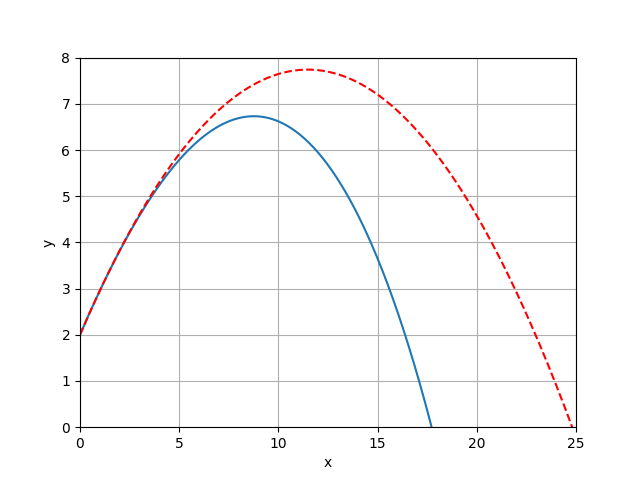
\includegraphics[width=0.6\textwidth]{fig2_43.png}
    \captionsetup{width=0.8\textwidth}
    \caption{Trajectory of a basketball thrown from a height of 2 m with an initial velocity $v_o$
    and subject to quadratic drag (solid curve). In a vacuum, the trajectory is given by the dashed
    curve.}
    \label{fig:2_43}
\end{figure} 
\begin{verbatim}
    range =  17.741443936603282
    range_vac =  24.844292311959776
\end{verbatim}

in a vacuum, the equations of motion are
\begin{align*}
    x &= v_{xo} t \\
    y &= y_o + v_{yo} t - \frac{1}{2} g t^2
\end{align*}

(b) The distance traveled in the horizontal direction before hitting the ground is $x = 17.7$ m. In
a vacuum, the distance traveled is $x = 24.8$ m.

\paragraph{2.45} (a) Using Euler's relation (2.76), prove that any complex number $z= x+iy$ can be
written in the form $z=re^{i\theta}$. (b) Write $z = 3 + 4i$ in the form $z = re^{i\theta}$.
(c) Write $z = 2e^{-i\pi/3}$ in the form $x + iy$.
\barh 
(a) Using polar coordinates $x = r\cos\theta$ and $y = r\sin\theta$
\begin{align*}
    z = x + iy = r\cos\theta + i r\sin\theta = r(\cos\theta + i\sin\theta) = re^{i\theta}
\end{align*}
$r$ and $\theta$ relate to the points on the unit circle in the complex plane

(b) Let $r = \sqrt{x^2 + y^2}$ and $\theta = \arctan(y/x)$ with $x=3$ and $y=4$
\begin{equation*}
        r = \sqrt{3^2 + 4^2} = 5 \qand \theta = \arctan(4/3) = \qty{0.93}{\radian}
\end{equation*}
hence $z = 5 e^{0.93i}$
(c) Let $r = 2$ and $\theta = -\pi/3$
\begin{align*}
    x &= r\cos\theta = 2\cos(-\pi/3) = 1 \\
    y &= r\sin\theta = 2\sin(-\pi/3) = -\sqrt{3} \\
    z &= 1 - i\sqrt{3}
\end{align*}

\paragraph{2.47} For each of the following two pairs of numbers compute $z+w$, $z-w$, $zw$, and 
$z/w$. (a) $z=6+8i$ and $w=3-4i$ (b) $z=8e^{i\pi/3}$ and $w=4e^{i\pi/6}$
\barh 
(a) With $z=10e^{0.93i}$ and $w=5e^{-0.93i}$ where $\theta = \arctan(4/3) = \qty{0.93}{\radian}$
\begin{align*}
    z+w &= 6+8i + 3-4i = 9+4i \\
    z-w &= 6+8i - (3-4i) = 3+12i \\
    zw &= (10e^{i\theta})(5e^{-i\theta}) = 50 \\ 
    \frac{z}{w} &= \frac{6+8i}{3-4i} = \frac{6+8i}{3-4i} \frac{3+4i}{3+4i} = \frac{-14+48i}{25} 
        = -0.56 + 1.92i \\
    \qor \\
    \frac{z}{w} &= \frac{10e^{i\theta}}{5e^{-i\theta}} = 2e^{2i\theta} = 2e^{1.86i} = -0.56 + 1.92i
\end{align*}
(b) With $z=4 + 4\sqrt{3}i$ and $w=2\sqrt{3} + 2i$
\begin{align*}
    z+w &= (4+2\sqrt{3}) + (4\sqrt{3} + 2)i \\
    z-w &= (4-2\sqrt{3}) + (4\sqrt{3} - 2)i \\
    zw &= 8e^{i\pi/3}4e^{i\pi/6} = 32e^{i\pi/2} = 32i \\
    \frac{z}{w} &= \frac{8e^{i\pi/3}}{4e^{i\pi/6}} = 2e^{i\pi/6} = \sqrt{3} + i
\end{align*}

\paragraph{2.49} Consider the complex number $z=e^{i\theta}=\cos{\theta} + i\sin{\theta}$. (a) By
evaluating $z^2$ two different ways, prove the trig identities $\cos{2\theta}=\cos^2\theta - 
\sin^2\theta$ and $\sin{2\theta}=2\sin\theta\cos\theta$. (b) Use the same technique to find
corresponding identities for $\cos{3\theta}$ and $\sin{3\theta}$.
\barh 
(a) 
\begin{align*}
    z^2 &= e^{i\theta}e^{i\theta} = e^{i2\theta} = \cos{2\theta} + i\sin{2\theta} \\
    &= (\cos{\theta} + i\sin{\theta})(\cos{\theta} + i\sin{\theta}) \\
    &= (\cos^2\theta - \sin^2\theta) + (2\cos\theta\sin\theta) i
\end{align*}
Equating the real and imaginary parts
\begin{align*}
    \cos{2\theta} &= \cos^2\theta - \sin^2\theta \\
    \sin{2\theta} &= 2\cos\theta\sin\theta
\end{align*}
(b)
\begin{align*}
    z^3 &= e^{i\theta}e^{i\theta}e^{i\theta} = e^{i3\theta} = \cos{3\theta} + i\sin{3\theta} \\
    &= (\cos{\theta} + i\sin{\theta})(\cos{2\theta} + i\sin{2\theta}) \\
    &= (\cos{\theta} + i\sin{\theta})(\cos^2\theta - \sin^2\theta + i2\cos\theta\sin\theta) \\
    &= (\cos^3\theta - 3\cos\theta\sin^2\theta) + i(3\cos^2\theta\sin\theta - \sin^3\theta)
\end{align*}
Equating the real and imaginary parts
\begin{align*}
    \cos{3\theta} &= \cos^3\theta - 3\cos\theta\sin^2\theta \\
    \sin{3\theta} &= 3\cos^2\theta\sin\theta - \sin^3\theta
\end{align*}

\paragraph{2.51} Use the series definition (2.72) of $e^z$ to prove that $e^ze^w=e^{z+w}$.
\barh 
Grouping each term of $z^nw^m$ where $n + m = p$. 
\begin{align*}
    e^ze^w &= \quantity[1 + z + z^2/2! + \dotsm] \quantity[1 + w + w^2/2! + \dotsm] \\
    &= \quantity[1 + (z+w) + \frac{1}{2!}(z^2 + 2zw + w^2)
        + \frac{1}{3!}(z^3 + 3z^2w + 3zw^2 + w^3)] + \dotsm
\end{align*}
The coefficient $1/N!$ in each term are factored out by $1/(N-1)! = N/N!$ e.g. $z^2w/2! =3z^2w/3!$.
Each term is a binomial expansion of $(z+w)^p$ where the first term is $p=0$, the second is $p=1$
etc. Hence
\begin{align*}
    e^ze^w &= \quantity[1 + (z+w) + \frac{1}{2!}(z+w)^2 + \frac{1}{3!}(z+w)^3 + \dotsm] \\
    &= e^{z+w}
\end{align*}
Q.E.D.

\paragraph{2.53} A charged particle of mass $m$ and charge $q$ moves in uniform electric and
magnetic fields, $\vb{E}$ and $\vb{B}$, both pointing in the $z$ direction. The net force on the
particle is $\vb{F} = q(\vb{E} + \vb{v} \cp \vb{B})$. Write down the equation of motion into its 
three components and solve the equations.
\barh 
The components of each vector are
\begin{align*}
    \vb{v} = (v_x,v_y,v_z) \qquad \vb{E} = (0,0,E) \qquad \vb{B} = (0,0,B)
        \qquad \vb{v}\cp\vb{B} = (v_yB, -v_xB, 0)
\end{align*}
The equation of motion is written as
\begin{align*}
    \dot{v}_x &= \omega v_y \\
    \dot{v}_y &= -\omega v_x \\
    m \dot{v}_z &= qE
\end{align*}
where $\omega = qB/m$ is the cyclotron frequency. Using the complex number $\eta = v_x + iv_y$ the
solution is in the general form
\begin{align*}
    \eta = Ae^{-iwt}
\end{align*}
where $A$ is a constant. The general solution for $x$ and $y$ are the real and imaginary parts of
$\xi=x+iy$ and constant $C=x_o+iy_o$ given by (2.80)
\begin{align*}
    \xi &= Ce^{-iwt}\\
    &= (x_o + iy_o)e^{-iwt} \\
    &= (x_o + iy_o) \quantity(\cos(\omega t) - i\sin(\omega t)) \\
    &= (x_o\cos(\omega t) + y_o\sin(\omega t)) + i(y_o\cos(\omega t) - x_o\sin(\omega t)) \\
\end{align*}
The solution for $x$ and $y$ are
\begin{align*}
    x &= x_o\cos(\omega t) + y_o\sin(\omega t) \\
    y &= y_o\cos(\omega t) - x_o\sin(\omega t)
\end{align*}

Solving for the motion in the $z$ direction
\begin{align*}
    \dot{v}_z &= \frac{qE}{m} \\
    v_z &= \frac{qE}{m} t + v_{zo} \\
    z &= \frac{qE}{2m} t^2 + v_{zo} t + z_o
\end{align*}
The particle moves in a circular path in the $xy$ plane with an increaseing velocity in the $z$
direction which combine to form a helix with increasing pitch in 3D space.

\paragraph{2.55} A charged particle of mass $m$ and charge $q$ moves in uniform electric and
magnetic fields, $\vb{E}$ pointing in the $y$ direction and $\vb{B}$ in the $z$ direction (an 
arrangement called "crossed E and B fields"). Suppose the particle is initially at the origin and is
given a kick at time $t = 0$ along the $x$ axis with $v_x = v_{xo}$ (positive or negative). (a) Write
down the equation of motion for the particle and resolve it into its three components. Show that the
motion remains in the plane $z = 0$. (b) Prove that there is a unique value of $v_{xo}$, called
drift speed $v_{dr}$, for which the particle moves undeflected through the fields. (This is the
basis of velocity selectors, which select particles traveling at one chosen speed froma beam with
many different speeds.) (c) Solve the equations of motion to give the particle's velocity as a
function of $t$, for arbitrary values of $v_{xo}$ (d) Integrate the velocity to find the position as
a function of $t$ and sketch the trajectory for various values of $v_{xo}$.
\barh 
(a) The components of each vector are
\begin{align*}
    \vb{v} = (v_x,v_y,v_z) \qquad \vb{E} = (0,E,0) \qquad \vb{B} = (0,0,B)
        \qquad \vb{v}\cp\vb{B} = (v_yB, v_xB, 0)
\end{align*}
The equation of motion is written as
\begin{align*}
    \dot{v}_x &= \omega v_y \\
    \dot{v}_y &= -\omega v_x + \frac{E\omega}{B} \\
    \dot{v}_z &= 0
\end{align*}
Since $\dot{v}_z = 0$, the motion remains in the plane $z = 0$.

(b) An undeflected particle will have $\dot{v}_y = 0$ and $\dot{v}_x = 0$ which is solved by
\begin{align*}
    0 = \omega v_y \qand 0 = -\omega v_x + \frac{E\omega}{B} \\
    v_y = 0 \qand v_x = \frac{E}{B}
\end{align*}
The drift speed is $v_{dr} = E/B$ which is constant and equivalent to the initial velocity $v_{xo}$.

(c) Solving the first two equations of motion by substituting $v_u = v_x - v_{dr}$ and 
$\dot{v}_u = \dot{v}_x$
\begin{align*}
    \dot{v}_u &= \omega v_y \\
    \dot{v}_y &= -\omega v_u
\end{align*}
which is the same as the equations of motion in Problem (2.53). The general solution is a complex
number $\eta = Ae^{-iwt}$. $A$ is then given by the initial conditions at $t=0$ which is
\begin{align*}
    A = v_{uo} + iv_{yo} = v_{xo} - v_{dr}
\end{align*}
This gives the solution on the complex plane which can be decomposed into its $x$ and $y$ components
\begin{align*}
    \eta &= (v_{xo} - v_{dr})e^{-iwt} \\
    v_u + iv_y &= (v_{xo}-v_{dr}) \quantity(\cos(\omega t) - i\sin(\omega t))
\end{align*}
The solution for $v_x$, rewritten using $v_x = v_u + v_{dr}$, and $v_y$ are
\begin{align*}
    v_x &= (v_{xo}-v_{dr})\cos(\omega t) + v_{dr}\\
    v_y &= -(v_{xo}-v_{dr})\sin(\omega t)
\end{align*}
Defining $R=(v_{xo}-v_{dr})/\omega$ the equations are simplified to
\begin{align*}
    v_x &= R\omega \cos(\omega t) + v_{dr}\\
    v_y &= -R\omega \sin(\omega t)
\end{align*}
(d) integrating from time 0 to $t$ to solve for the $x$ position
\begin{align*}
    \int_{0}^{x}\dd{x} &= x_o + \int_{0}^{t} R\omega \cos(\omega t) + v_{dr} \dd{t}\\
    x &= \eval{R\sin(\omega t) + + v_{dr}t}_{0}^{t} + x_o \\
    x &= R \sin(\omega t) + v_{dr}t + x_o\\
\end{align*}
same for the $y$ position
\begin{align*}
    y &= y_o + \int_{0}^t -R\omega \sin(\omega t) \dd{t} \\
    &= \eval{R\cos(\omega t)}_{0}^{t} + y_o\\
    y &= R\cos(\omega t) + R + y_o
\end{align*}
solving for the initial conditions $x_o$ and $y_o$ using $x(0) = 0$ and $y(0) = 0$
\begin{align*}
    x_o &= 0 \\
    y_o &= -2R
\end{align*}
The equation for the trajectory is
\begin{align*}
    x &= R \sin(\omega t) + v_{dr}t \\
    y &= R\cos(\omega t) - R \\
    \qor \\
    x &= \frac{v_{xo}-v_{dr}}{\omega} \sin(\omega t) + v_{dr}t \\
    y &= \frac{v_{xo}-v_{dr}}{\omega} (\cos(\omega t) - 1)
\end{align*}
with $\omega=1$ and $v_{dr} = 1$ the trajectory for various values of $v_{xo}$ is shown by Figure
\ref{fig:2_55}
\begin{figure}[ht]
    \centering
    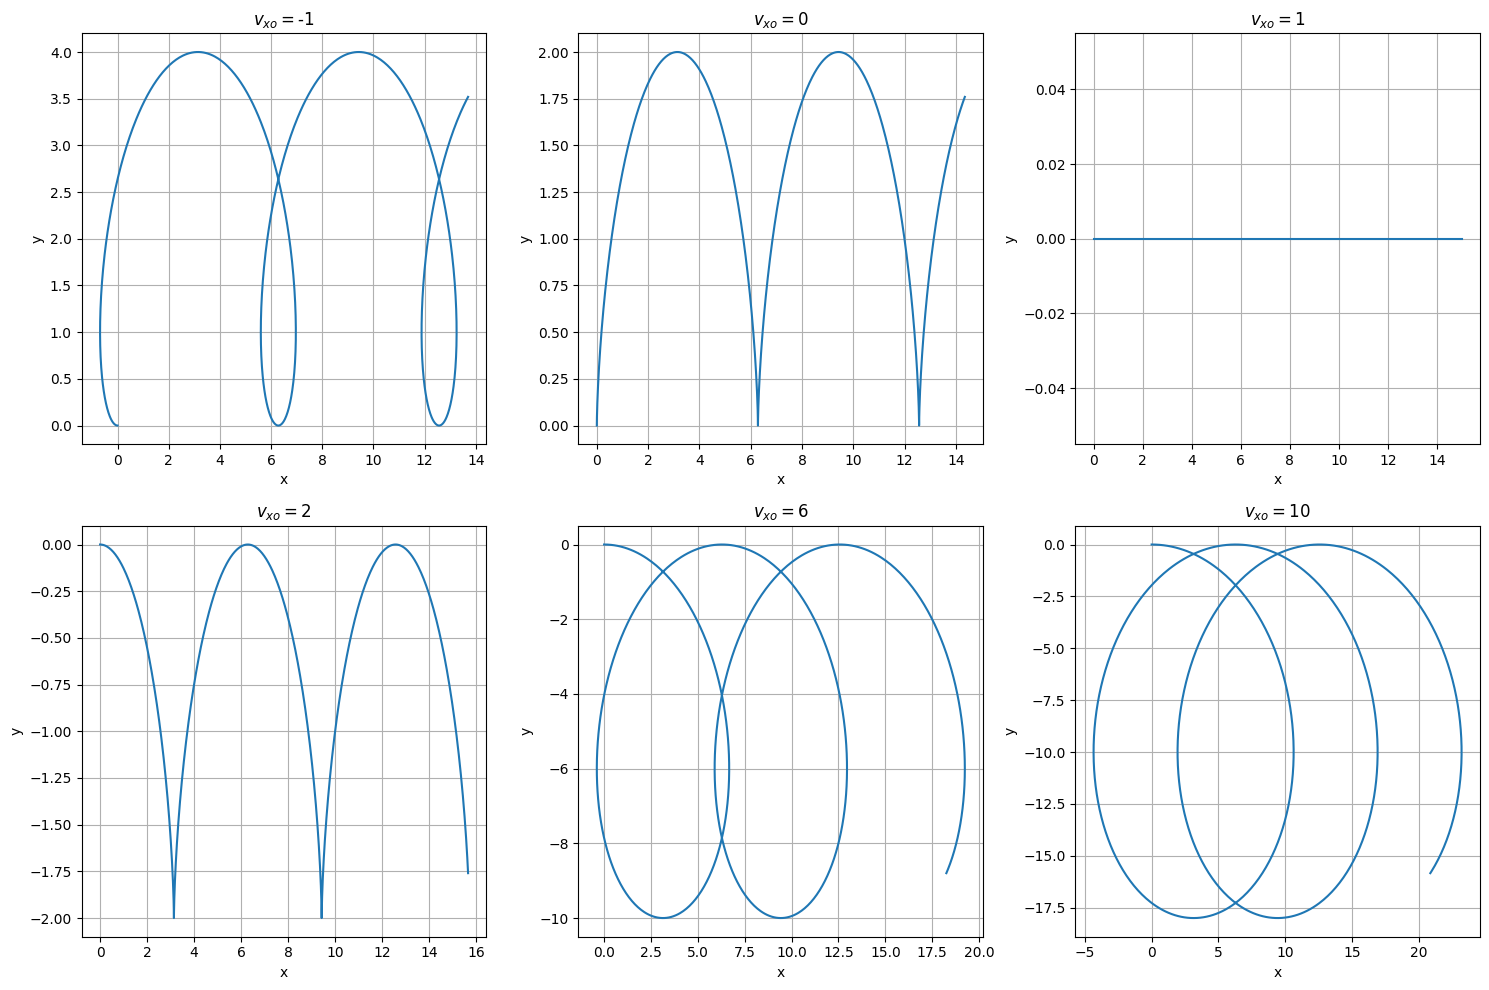
\includegraphics[width=0.6\textwidth]{fig2_55.png}
    \captionsetup{width=0.8\textwidth}
    \caption{Trajectory of a charged particle in crossed electric and magnetic fields with intial
    velocities $v_{xo}= \numlist{-1;0;1;2;6;10}$ m/s. When the initial velocity is equivalent to the
    drift speed $v_{dr} = 1$, the particle moves undeflected.}
    \label{fig:2_55}
\end{figure}
\end{document}